\documentclass[a4paper,11pt]{article}

% Packages
\usepackage[utf8]{inputenc}
\usepackage[T1]{fontenc}
\usepackage{graphicx}
\usepackage{amsmath,amssymb}
\usepackage{booktabs}
\usepackage{multirow}
% Add natbib for author-year or numeric citations
\usepackage{hyperref}
\usepackage{url}
\usepackage[margin=2.5cm]{geometry}
\usepackage{caption}
\usepackage{subcaption}
\usepackage{longtable}
\usepackage{rotating}
\usepackage{xurl}
\usepackage{hyperref}
\urlstyle{tt}
\usepackage[style=nature]{biblatex}
\addbibresource{bibliography.bib}
\newcommand{\feat}[1]{\texttt{\nolinkurl{#1}}}




\begin{document}


% Custom EPFL front page
\begin{titlepage}
    \centering
    % \vspace*{1cm}
    \textbf{\large
    ECOLE POLYTECHNIQUE FEDERALE DE LAUSANNE\\
    SCHOOL OF LIFE SCIENCES
    }
    \vspace{0.5cm}

    \begin{figure}[h]
        \centering
        
\includegraphics[width=0.5\linewidth]{figures/logo-epfl.png}
    \end{figure}

    {\Large
    Master project in Life Sciences Engineering
    }

    \vspace{2cm}

    \textbf{
    {\large [THESIS TITLE]
    }}

    \vspace{1.5cm}
    \fbox{% 
        \parbox{1\textwidth}{
            \centering
            Carried out in the laboratory of [SUPERVISOR NAME]\\
            at [INSTITUTION/LABORATORY]\\
            Under the supervision of [CO-SUPERVISOR NAME]
        }
    }

    \vspace{2cm}
    Done by

    \vspace{0.5cm}
    \textbf{\Large [STUDENT NAME]}

    \vspace{1.5cm}
    Under the direction of\\ {}[EPFL SUPERVISOR NAME]\\

    \vspace{1cm}
    EPFL

    % \vspace{1cm}
    % External Expert \\
    % \small{(First and last names, title of your oral exam expert, if different from your lab supervisor in the foreign lab and already mentioned above)}

    \vfill
    LAUSANNE, EPFL 2025
\end{titlepage}


\newpage

\null
\thispagestyle{empty}

\newpage

\pagenumbering{roman}

\section*{Acknowledgements}
\addcontentsline{toc}{section}{Acknowledgements}

\bigskip

\noindent I thank [EXTERNAL SUPERVISOR NAME], [EPFL SUPERVISOR NAME], and [DAILY SUPERVISOR/POSTDOC NAME] for their guidance and support, my lab colleagues for a collaborative environment, and my family and friends for their encouragement throughout this work. \bigskip


\newpage

\null
\thispagestyle{empty}

\newpage

\section*{Abstract}
\addcontentsline{toc}{section}{Abstract}

\noindent This thesis addresses a broadly relevant problem in life sciences engineering and proposes a concise, reproducible, and data-driven approach for analyzing complex biological data. The objectives are to standardize the workflow, ensure transparent evaluation, and support practical use across related contexts.

\noindent We present a general pipeline that integrates preprocessing, statistical modeling, and machine learning, accompanied by clear reporting and open templates. The results highlight consistent patterns across datasets (without task-specific claims), and the contributions include a reusable framework, documented protocols, and guidance for future applications and extensions.

\newpage

\null
\thispagestyle{empty}


\newpage

\section*{Acronyms}
\addcontentsline{toc}{section}{Acronyms}

\begin{table}[htp!]
\centering
\label{tab:acronyms}
\begin{tabular}{ll}
\hline
\textbf{Acronym} & \textbf{Definition} \\
\hline
AI & Artificial Intelligence \\
API & Application Programming Interface \\
AUC & Area Under the Curve \\
CV & Cross Validation \\
DNA & Deoxyribonucleic Acid \\
EPFL & École Polytechnique Fédérale de Lausanne \\
FDR & False Discovery Rate \\
GPU & Graphics Processing Unit \\
HPC & High-Performance Computing \\
ML & Machine Learning \\
mRNA & messenger Ribonucleic Acid \\
PCA & Principal Component Analysis \\
PCR & Polymerase Chain Reaction \\
QC & Quality Control \\
RF & Random Forest \\
RNA & Ribonucleic Acid \\
ROC & Receiver Operating Characteristic \\
SLS & School of Life Sciences \\
SVM & Support Vector Machine \\
UI & User Interface \\
\hline
\end{tabular}
\end{table}


\newpage

\null
\thispagestyle{empty}

\newpage

\tableofcontents

\newpage

\null
\thispagestyle{empty}

\newpage


\pagenumbering{arabic}

\section{Introduction}

\noindent This template provides a brief, generic introduction suitable for an EPFL School of Life Sciences master thesis. It motivates the need for clear, reproducible, and data\,driven analyses without binding the thesis to a specific application.

\noindent The following chapters outline a general methodology, present representative results, and discuss implications and limitations. Replace this placeholder with project\,specific objectives, datasets, and contributions.

\bigskip

\noindent Figure~\ref{fig:cell-overview} shows how to insert and reference a single image. In Figure~\ref{fig:cell-subfigures}, panels~\subref{fig:cell-sub-a} and~\subref{fig:cell-sub-b} demonstrate subfigures and cross\,referencing to specific panels.

\begin{figure}[h]
  \centering
  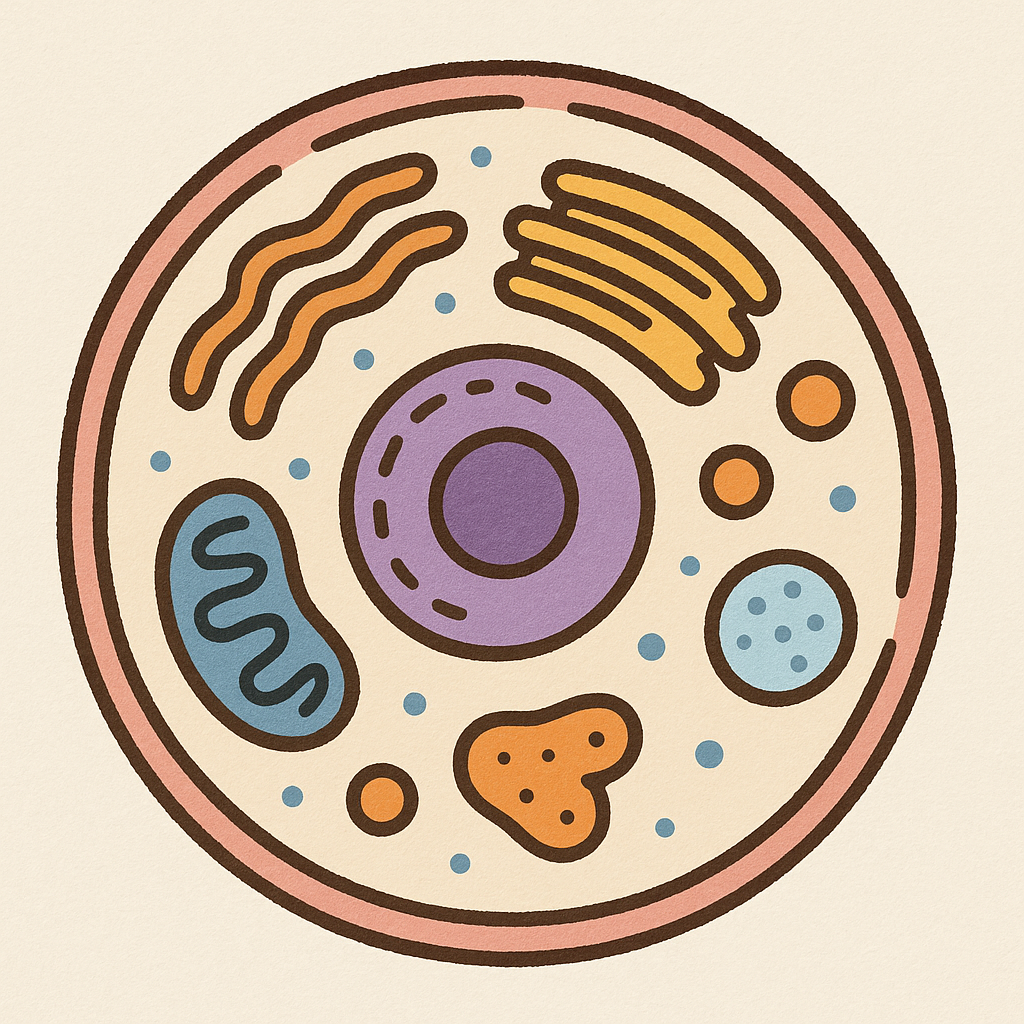
\includegraphics[width=0.48\textwidth]{figures/cell.png}
  \caption{Overview illustration: a mother cell giving rise to two daughter cells.}
  \label{fig:cell-overview}
\end{figure}

\begin{figure}[h]
  \centering
  \begin{subfigure}{0.48\textwidth}
    \centering
    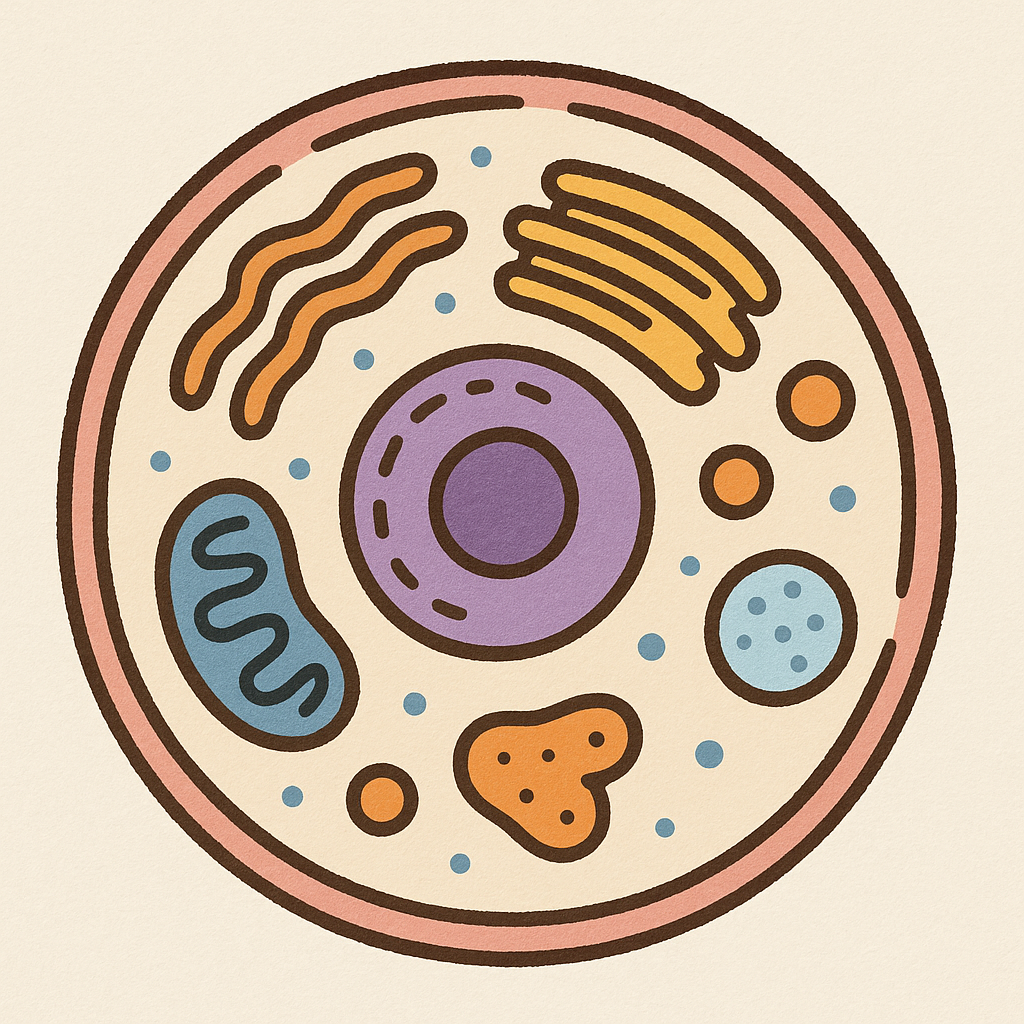
\includegraphics[width=\linewidth]{figures/cell.png}
    \caption{Daughter Cell 1.}
    \label{fig:cell-sub-a}
  \end{subfigure}\hfill
  \begin{subfigure}{0.48\textwidth}
    \centering
    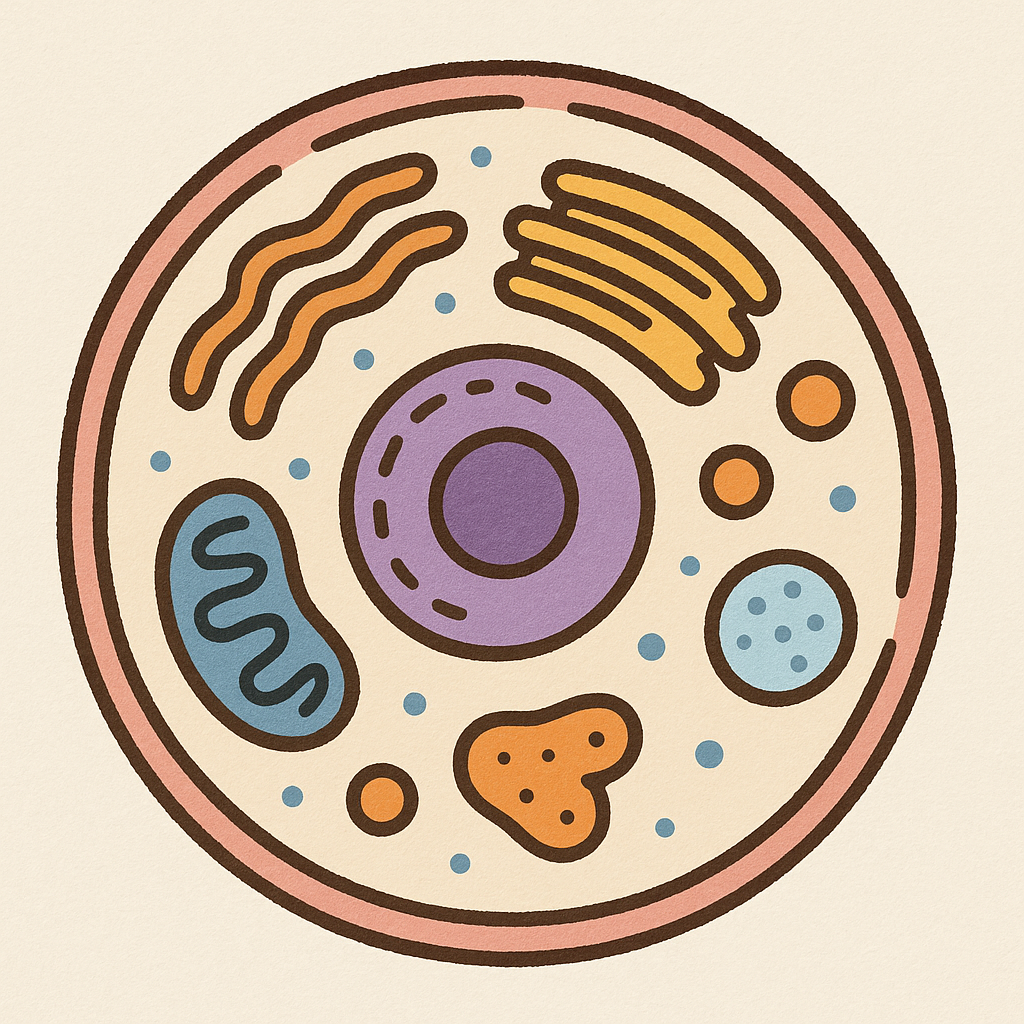
\includegraphics[width=\linewidth]{figures/cell.png}
    \caption{Daughter Cell 2.}
    \label{fig:cell-sub-b}
  \end{subfigure}
  \caption{Subfigure example: the same image reused to illustrate two conceptual panels.}
  \label{fig:cell-subfigures}
\end{figure}

\newpage

\section{Materials and Methods}

\noindent This section outlines a concise, generic workflow suitable for life sciences data analysis. It typically includes data collection or selection, preprocessing and quality control, feature engineering, model development, and evaluation under reproducible settings.

\noindent Replace this placeholder with project\,specific details: datasets and inclusion criteria, preprocessing steps, models and hyperparameters, validation procedures, software and versions, and any ethical or data\,use considerations.


\subsection{Example of Citation Method}

\noindent Reproducible computational research and rigorous data stewardship are foundational to modern life sciences. Adopting the FAIR Guiding Principles ensures that datasets and metadata are findable, accessible, interoperable, and reusable across studies and platforms \parencite{wilkinson2016fair}. Following established best practices for reproducibility—such as version control, scripted analyses, exact environment capture, and public archiving—reduces analytic ambiguity and supports transparent validation \parencite{sandve2013reproducible}. In parallel, advances in machine learning provide scalable tools for pattern discovery and prediction from high-dimensional biological measurements, but their utility depends critically on well-curated, shareable data and reproducible workflows \parencite{tarca2007mlbio}.



\newpage

\section{Results}

\noindent This section summarizes representative outcomes at a high level, focusing on patterns aligned with the study objectives and on robustness checks (e.g., cross\,validation, external validation, and uncertainty estimates).

\noindent Replace this placeholder with project\,specific findings: key metrics and confidence intervals, brief references to figures/tables, and observations relevant to the research questions. Avoid over\,claiming; note caveats that affect interpretation and generalizability.

\bigskip

\noindent Table~\ref{tab:results-csv} illustrates how to import a table from a CSV file (see \texttt{tables/results\_example.csv}). Update the CSV and recompile to refresh the table.

\begin{table}[h]
  \centering
  \caption{Dummy performance metrics imported from CSV.}
  \label{tab:results-csv}
  \csvautobooktabular{tables/results_example.csv}
\end{table}

\noindent Large tables can overflow the page. Table~\ref{tab:too-wide-example} shows an example of a table that is too wide. Table~\ref{tab:wide-example} shows how to wrap a wide table with :


\begin{center}
    \verb|\resizebox{\textwidth}{!}{...}| 
\end{center}

\noindent so it fits the page width.

\begin{table}[htbp]
    \centering
    \caption{Example of a wide table resized to fit the page width.}
    \label{tab:too-wide-example}
    \begin{tabular}{lccccccccccccccc}
        \toprule
        ID & F1 & F2 & F3 & F4 & F5 & F6 & F7 & F8 & F9 & F10 & F11 & F12 & F13 & F14 & F15 \\
        \midrule
        A01 & 0.12 & 0.34 & 0.56 & 0.78 & 0.91 & 0.45 & 0.67 & 0.89 & 0.23 & 0.35 & 0.44 & 0.52 & 0.68 & 0.72 & 0.81 \\
        A02 & 0.22 & 0.31 & 0.58 & 0.74 & 0.88 & 0.41 & 0.63 & 0.85 & 0.27 & 0.39 & 0.48 & 0.54 & 0.70 & 0.74 & 0.83 \\
        A03 & 0.18 & 0.29 & 0.61 & 0.72 & 0.86 & 0.47 & 0.66 & 0.83 & 0.25 & 0.37 & 0.46 & 0.50 & 0.66 & 0.71 & 0.80 \\
        A04 & 0.20 & 0.33 & 0.59 & 0.76 & 0.90 & 0.43 & 0.65 & 0.87 & 0.21 & 0.31 & 0.42 & 0.49 & 0.64 & 0.69 & 0.78 \\
        \bottomrule
    \end{tabular}
\end{table}


\begin{table}[htbp]
  \centering
  \caption{Example of a wide table resized to fit the page width.}
  \label{tab:wide-example}
  \resizebox{\textwidth}{!}{%
    \begin{tabular}{lccccccccccccccc}
      \toprule
      ID & F1 & F2 & F3 & F4 & F5 & F6 & F7 & F8 & F9 & F10 & F11 & F12 & F13 & F14 & F15 \\
      \midrule
      A01 & 0.12 & 0.34 & 0.56 & 0.78 & 0.91 & 0.45 & 0.67 & 0.89 & 0.23 & 0.35 & 0.44 & 0.52 & 0.68 & 0.72 & 0.81 \\
      A02 & 0.22 & 0.31 & 0.58 & 0.74 & 0.88 & 0.41 & 0.63 & 0.85 & 0.27 & 0.39 & 0.48 & 0.54 & 0.70 & 0.74 & 0.83 \\
      A03 & 0.18 & 0.29 & 0.61 & 0.72 & 0.86 & 0.47 & 0.66 & 0.83 & 0.25 & 0.37 & 0.46 & 0.50 & 0.66 & 0.71 & 0.80 \\
      A04 & 0.20 & 0.33 & 0.59 & 0.76 & 0.90 & 0.43 & 0.65 & 0.87 & 0.21 & 0.31 & 0.42 & 0.49 & 0.64 & 0.69 & 0.78 \\
      \bottomrule
    \end{tabular}%
  }
\end{table}

\newpage

\section{Discussion}

\noindent This section provides a concise interpretation of the results in relation to the study objectives. Emphasis is placed on what the findings suggest, how robust they appear under the chosen validation strategy, and how they fit within a broader life sciences context.

\noindent Replace this placeholder with project\,specific discussion points: main takeaways, practical implications, limitations (data, methods, assumptions), and prioritized future directions. Clearly distinguish evidence\,based claims from speculation, and note any dependencies that may affect generalizability.

\newpage

\section{Conclusion}

\noindent This section provides a brief synthesis of the work and its contributions. In its generic form, it highlights that a reproducible, data\,driven methodology was presented, representative results were obtained, and practical lessons were drawn for life sciences applications.

\noindent Replace this placeholder with project\,specific takeaways: summarize the main findings without restating all details, note limitations that matter most, and outline concrete next steps (e.g., additional validation, broader datasets, or methodological extensions).

\newpage

\section{Supplementary Material}

\noindent This section provides space for additional material that supports the main text, such as extended methods, extra figures/tables, or robustness checks. Include only information that aids reproducibility or clarifies key results.

\noindent Replace this placeholder with project\,specific supplementary items (e.g., detailed parameter settings, expanded validation, or additional results). Reference supplementary items from the main text where appropriate.

\newpage
\null
\newpage

\printbibliography

\end{document}
